\section{引言}
\label{sec:intro}

知识蒸馏（KD）已成为深度神经网络压缩的标准技术，使得轻量级模型能够部署在资源受限的平台上\cite{hinton2015distilling}。在目标检测领域，KD允许轻量级学生网络从更大、更准确的教师模型获取知识，在降低计算成本的同时达到可比的性能\cite{chen2017learning, dai2021general}。然而，KD在恶劣视觉条件下的可靠性——特别是由雾、霾或雨导致的可见度退化——仍是一个关键但未充分解决的问题。

近期研究已记录到KD在域偏移和恶劣天气条件下性能下降的现象\cite{guo2021meets, du2022learning}。但\emph{为什么}会失效仍不清楚。KD失效是因为教师-学生分布对齐被打破？是因为教师预测在退化输入下不确定性增加？还是因为可见度破坏从根本上改变了知识转移所依赖的视觉线索？如果不理解主导失效机制，开发鲁棒KD方法的努力可能只是在治标而非治本。

本文通过机制驱动的实证研究来解决这一空白。我们不是提出又一种KD变体，而是系统地剖析现有KD方法在可见度退化下失效的原因。我们的方法采用结构化的分支级分析：分离四种不同的KD机制——logit蒸馏、特征蒸馏、注意力蒸馏和定位蒸馏——并在受控的可见度等级谱上评估它们的行为。

本研究得出三个主要发现。\textbf{第一}，我们确认分支级性能结构确实存在：不同KD分支对可见度退化的响应不同，logit蒸馏尽管文献中广泛使用却被证明并非最优，而定位蒸馏表现出相对鲁棒性。\textbf{第二}，我们实证检验了三种假设的失效机制。分布错配和不确定性放大虽然是常被援引的解释，但与KD增益的相关性弱且统计不显著（$|r|<0.5$，$p>0.7$），在本设置中不足以解释观测到的退化。\textbf{第三}，也是最关键的，我们发现遮挡——可见度退化的具体可测成分——与定位性能呈现强负相关（$r=-0.989$，$p=0.0015$），是所测试机制中最直接得到证据支持的因素。

这些发现具有重要的方法论意义。我们的分析表明，logit KD失效不太可能仅通过简单超参数调整解决。遮挡与定位性能之间的强相关性提示：针对恶劣条件的未来KD方法应优先处理遮挡和空间信息损失机制，而非仅关注分布对齐或不确定性校准。

本文的贡献包括：
\begin{itemize}
    \item 首个控制性实证研究，理清可见度退化下KD失效的竞争性解释，建立"观测-机制验证"结构化框架；
    \item 证明广泛假设的机制（分布错配、不确定性放大）不足以解释观测到的KD退化，挑战文献中的主流直觉；
    \item 识别遮挡——可见度退化的具体可测成分——为所测试机制中最直接得到支持的因素；
    \item 证明KD失效不能归因于简单超参数调优，表明需要架构层面而非配置层面的解决方案。
\end{itemize}

\Cref{fig:conceptual_framework}展示了我们的机制驱动分析框架。

\begin{figure*}[htbp]
\centering
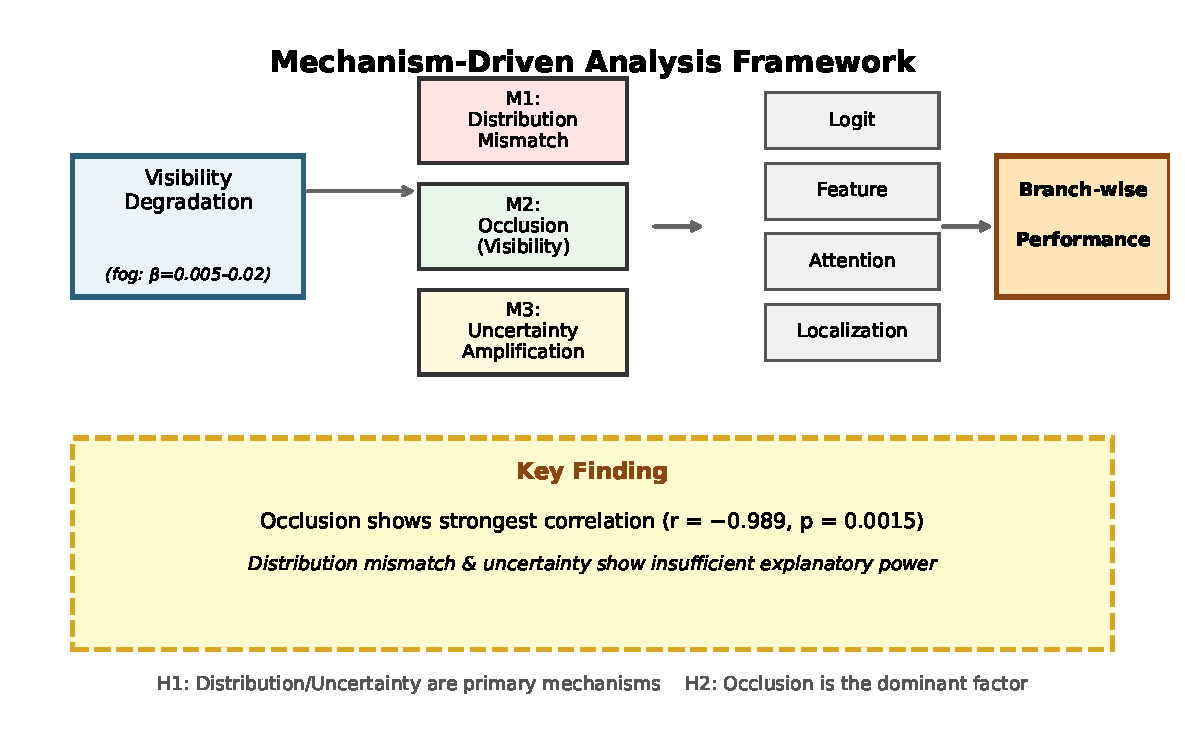
\includegraphics[width=0.9\textwidth]{figures/figure1_conceptual.pdf}
\caption{机制驱动分析框架。我们在四个KD分支上评估三种假设机制（M1、M2、M3），以识别所测试机制中最强得到证据支持的因素。研究发现，遮挡（M2内）是最直接得到支持的机制，而分布错配和不确定性放大在本设置中解释力不足。}
\label{fig:conceptual_framework}
\end{figure*}

本文余下部分组织如下。\cref{sec:related}回顾KD在检测和域偏移下的相关工作。\cref{sec:setup}描述实验设计和分支级框架。\cref{sec:observation}呈现建立分支级性能结构的观测结果。\cref{sec:mechanism}详细分析机制及支持遮挡为最相关因素的证据。\cref{sec:discussion}讨论意义和局限性，\cref{sec:conclusion}总结并展望未来方向。
